% =====================================================================
%  Лабораторная работа №6. Методы решения дифференциальных уравнений.
%  Вариант 4: y'' - x*y' + 2*y = x + 1,
%             y(0,9) - 0,5*y'(0,9) = 2, y(1,2) = 1.
%
%  Сборка (любой из вариантов):
%      pdflatex  BastrakovReport.tex
%      xelatex   BastrakovReport.tex
%      lualatex  BastrakovReport.tex
%  (запускать два раза — для оглавления и перекрёстных ссылок)
% =====================================================================
\documentclass[14pt,a4paper]{extarticle}

% - Поддержка кириллицы: pdfLaTeX (T2A) либо XeLaTeX/LuaLaTeX (fontspec) -
\usepackage{iftex}
\ifPDFTeX
    \usepackage[T2A]{fontenc}
    \usepackage[utf8]{inputenc}
    \usepackage[russian]{babel}
    \usepackage{tempora}
    \usepackage{listingsutf8}
\else
    \usepackage{fontspec}
    \usepackage{polyglossia}
    \setdefaultlanguage{russian}
    \setotherlanguage{english}
    \IfFontExistsTF{Liberation Serif}%
        {\setmainfont{Liberation Serif}}%
        {\IfFontExistsTF{PT Serif}%
            {\setmainfont{PT Serif}}%
            {\setmainfont{TeX Gyre Termes}}}
    \IfFontExistsTF{DejaVu Sans Mono}%
        {\setmonofont{DejaVu Sans Mono}}%
        {\IfFontExistsTF{Liberation Mono}%
            {\setmonofont{Liberation Mono}}%
            {\setmonofont{TeX Gyre Cursor}}}
\fi

% - Математика, графика, оформление -----------
\usepackage{amsmath,amssymb}
\usepackage{graphicx}
\usepackage{geometry}
\usepackage{booktabs}
\usepackage{array}
\usepackage{float}
\usepackage{caption}
\usepackage{indentfirst}
\usepackage{xcolor}
\usepackage[hidelinks]{hyperref}

\geometry{a4paper,left=3cm,right=1.5cm,top=2cm,bottom=2cm}
\graphicspath{{graphics/img/}}

\captionsetup{labelsep=endash,justification=centering}
\setlength{\parindent}{1.25cm}
% Запас на растяжение строк: в XeLaTeX могут отсутствовать русские
% шаблоны переносов, поэтому длинные слова иначе вылезают за поля.
\setlength{\emergencystretch}{3em}
\tolerance=2000
\renewcommand{\arraystretch}{1.15}
\renewcommand{\labelenumi}{\arabic{enumi})}

\begin{document}

% =====================================================================
%  Титульный лист
% =====================================================================
\begin{titlepage}
    \centering
    \large
    Министерство образования и науки РФ\\[0.3cm]
    Пермский национальный исследовательский политехнический университет\\[0.3cm]
    Электротехнический факультет\\[0.3cm]
    Кафедра "Информационные технологии и автоматизированные системы"

    \vspace{3.5cm}
    {\Large Информатика в приложении к отрасли}\\[0.4cm]
    {\Large\bfseries Лабораторная работа № 6}\\[0.6cm]

    Тема: "Методы решения дифференциальных уравнений"\\[0.2cm]
    Вариант 4

    \vspace{4.5cm}
    \begin{flushleft}
        \large
        Выполнил: студент группы РИС-25-2б \hfill Бастраков Данил\\[0.5cm]
        Проверил: профессор кафедры ИТАС \hfill Шварц К.~Г.\\[0.5cm]
        Дата: \underline{\hspace{3cm}} \hfill Подпись: \underline{\hspace{4cm}}
    \end{flushleft}

    \vfill
    Пермь\\ 2026
\end{titlepage}

\tableofcontents
\newpage

% =====================================================================
\section{Постановка задачи}
% =====================================================================

\textbf{Цель работы} --- численно решить краевую задачу для обыкновенного
дифференциального уравнения второго порядка методом конечных разностей
и реализовать решение полученной трёхдиагональной системы методом прогонки.

Вариант~4 задаёт уравнение
\begin{equation}
    y'' - x y' + 2y = x + 1, \qquad x \in [0{,}9;\, 1{,}2],
    \label{eq:ode}
\end{equation}
с краевыми условиями
\begin{equation}
    \begin{cases}
        y(0{,}9) - 0{,}5\,y'(0{,}9) = 2,\\
        y(1{,}2) = 1.
    \end{cases}
    \label{eq:bc}
\end{equation}
Шаг сетки по заданию $h=0{,}05$, число отрезков
$n=(1{,}2-0{,}9)/0{,}05=6$, узлы $x_i=0{,}9+0{,}05\,i$, $i=0,\ldots,6$.

Уравнение~\eqref{eq:ode} имеет вид (2.1) методических указаний:
$y''+p(x)y'+q(x)y=f(x)$, где
\begin{equation}
    p(x) = -x, \qquad q(x) = 2, \qquad f(x) = x+1 .
    \label{eq:coeff}
\end{equation}
Краевые условия~\eqref{eq:bc} соответствуют (2.2)--(2.3) при
$\alpha_0=1$, $\alpha_1=-0{,}5$, $A=2$, $\beta_0=1$, $\beta_1=0$, $B=1$.
По условию $\alpha_0+\alpha_1\ne0$ и $\beta_0+\beta_1\ne0$, задача
корректна. Точное решение в элементарных функциях не требуется: точность
контролируется невязкой разностной системы и сравнением решений на двух
сетках.

% =====================================================================
\section{Краткое описание метода}
% =====================================================================

\subsection{Конечно-разностная аппроксимация}

Внутренние узлы сетки $x_i$, $i=1,\ldots,n-1$, аппроксимируем производные
центральными разностями (2.4)--(2.5):
\begin{equation}
    y''(x_i) \approx \frac{y_{i+1}-2y_i+y_{i-1}}{h^2}, \qquad
    y'(x_i) \approx \frac{y_{i+1}-y_{i-1}}{2h} .
    \label{eq:diff}
\end{equation}
Подстановка~\eqref{eq:diff} в уравнение~\eqref{eq:ode} даёт разностное
уравнение
\begin{equation}
    \frac{y_{i+1}-2y_i+y_{i-1}}{h^2}
    + p(x_i)\frac{y_{i+1}-y_{i-1}}{2h}
    + q(x_i)y_i = f(x_i), \qquad i=1,\ldots,n-1,
    \label{eq:diff-eq}
\end{equation}
аппроксимирующее дифференциальное уравнение с погрешностью $O(h^2)$.
Умножая~\eqref{eq:diff-eq} на $h^2$ и деля на $1+0{,}5p(x_i)h$, получим
\begin{equation}
    a_i y_{i-1} - b_i y_i + y_{i+1} = d_i,
    \label{eq:three}
\end{equation}
где
\begin{equation}
    a_i = \frac{1-0{,}5p(x_i)h}{1+0{,}5p(x_i)h},\qquad
    b_i = \frac{2-q(x_i)h^2}{1+0{,}5p(x_i)h},\qquad
    d_i = \frac{h^2 f(x_i)}{1+0{,}5p(x_i)h}.
    \label{eq:abd}
\end{equation}
Краевые условия аппроксимируются односторонними разностями ($O(h)$):
\begin{equation}
    \left(\alpha_0-\frac{\alpha_1}{h}\right)y_0
      +\frac{\alpha_1}{h}y_1 = A,\qquad
    -\frac{\beta_1}{h}y_{n-1}
      +\left(\beta_0+\frac{\beta_1}{h}\right)y_n = B .
    \label{eq:bc-diff}
\end{equation}
В варианте~4 $\beta_1=0$, поэтому второе условие просто $y_6=1$.

\subsection{Метод прогонки}

Система~\eqref{eq:three},~\eqref{eq:bc-diff} имеет трёхдиагональную матрицу
порядка $n+1$. Решение ищется в виде (2.12):
\begin{equation}
    y_i = P_i y_{i+1} + Q_i, \qquad i=0,\ldots,n-1 .
    \label{eq:sweep-form}
\end{equation}
Из левого краевого условия:
\begin{equation}
    \begin{aligned}
        P_0 &= -\frac{\alpha_1}{\alpha_0 h-\alpha_1}
              = \frac{0{,}5}{0{,}05+0{,}5} = 0{,}90909091,\\
        Q_0 &= \frac{Ah}{\alpha_0 h-\alpha_1}
              = 0{,}18181818 .
    \end{aligned}
    \label{eq:sweep-start}
\end{equation}
Прямой ход (2.15):
\begin{equation}
    P_i = -\frac{1}{a_i P_{i-1}-b_i},\qquad
    Q_i = \frac{d_i-a_i Q_{i-1}}{a_i P_{i-1}-b_i},
    \qquad i=1,\ldots,n-1 .
    \label{eq:sweep-forward}
\end{equation}
Обратный ход начинается с правого краевого условия (2.16):
\begin{equation}
    y_n = \frac{Bh+\beta_1 Q_{n-1}}
               {\beta_0 h+\beta_1(1-P_{n-1})},
    \label{eq:sweep-last}
\end{equation}
после чего последовательно вычисляются
$y_{n-1},\,y_{n-2},\,\ldots,\,y_0$ по формуле~\eqref{eq:sweep-form}.
Знаменатели $a_iP_{i-1}-b_i$ здесь отрицательны и по модулю больше единицы,
поэтому прогонка устойчива.

\subsection{Ограничение на число массивов}

По заданию программа должна использовать не более трёх одномерных
массивов. Используются массивы $P$, $Q$ (прогоночные коэффициенты) и $Y$
(решение на мелкой сетке с шагом $h/2$). Коэффициенты $a_i,b_i,d_i$
вычисляются по формулам~\eqref{eq:abd} скалярами по мере обхода узлов.
Для сравнения сеток задача сначала решается на мелкой сетке, затем те же
массивы $P,Q$ переиспользуются для грубой сетки, а её значения помещаются
в не участвующую в обратном ходе часть массива $P$. Таким образом,
одновременно задействовано ровно три массива.

% =====================================================================
\section{Исходные данные}
% =====================================================================

Параметры читаются из файла \texttt{input.txt} (строки, начинающиеся
с~\texttt{\#}, являются комментариями). Файл содержит три числа:
\begin{equation}
    a = 0{,}9,\qquad b = 1{,}2,\qquad h = 0{,}05 .
    \label{eq:input}
\end{equation}
Вид уравнений~\eqref{eq:ode}--\eqref{eq:bc} фиксирован вариантом~4,
как и правая часть в лабораторной работе №~5 была фиксирована номером
варианта.

% =====================================================================
\section{Результаты вычислений}
% =====================================================================

\subsection{Коэффициенты разностной системы}

Для внутренних узлов $x_1,\ldots,x_5$ по формулам~\eqref{eq:abd}
получены коэффициенты, приведённые в табл.~\ref{tab:abd}
($p(x_i)=-x_i$, $q(x_i)=2$, $f(x_i)=x_i+1$).

\begin{table}[H]
    \centering
    \caption{Коэффициенты разностного уравнения}
    \label{tab:abd}
    \small
    \begin{tabular}{crrrr}
        \toprule
        $i$ & $x_i$ & $a_i$ & $b_i$ & $d_i$\\
        \midrule
        1 & $0{,}95$ & $1{,}04865557$ & $2{,}04353393$ & $0{,}00499360$\\
        2 & $1{,}00$ & $1{,}05128205$ & $2{,}04615385$ & $0{,}00512821$\\
        3 & $1{,}05$ & $1{,}05391528$ & $2{,}04878049$ & $0{,}00526316$\\
        4 & $1{,}10$ & $1{,}05655527$ & $2{,}05141388$ & $0{,}00539846$\\
        5 & $1{,}15$ & $1{,}05920206$ & $2{,}05405405$ & $0{,}00553411$\\
        \bottomrule
    \end{tabular}
\end{table}

\subsection{Прогоночные коэффициенты}

По формулам~\eqref{eq:sweep-start}--\eqref{eq:sweep-forward} вычислены
$P_i,Q_i$ (табл.~\ref{tab:sweep}). Коэффициенты $P_6,Q_6$ не используются:
$y_6$ определяется непосредственно правым краевым условием.

\begin{table}[H]
    \centering
    \caption{Прогоночные коэффициенты}
    \label{tab:sweep}
    \small
    \begin{tabular}{crrr}
        \toprule
        $i$ & $x_i$ & $P_i$ & $Q_i$\\
        \midrule
        0 & $0{,}90$ & $0{,}90909091$ & $0{,}18181818$\\
        1 & $0{,}95$ & $0{,}91725390$ & $0{,}17030750$\\
        2 & $1{,}00$ & $0{,}92433292$ & $0{,}16075352$\\
        3 & $1{,}05$ & $0{,}93056851$ & $0{,}15275974$\\
        4 & $1{,}10$ & $0{,}93613954$ & $0{,}14603837$\\
        5 & $1{,}15$ & $0{,}94118256$ & $0{,}14037742$\\
        \bottomrule
    \end{tabular}
\end{table}

\subsection{Значения решения в узлах сетки}

Обратный ход даёт значения $y_i$, приведённые в табл.~\ref{tab:solution}.
Решение монотонно убывает от $1{,}4193941690$ до $1$, причём правое
краевое условие выполнено точно.

\begin{table}[H]
    \centering
    \caption{Решение краевой задачи при $h=0{,}05$}
    \label{tab:solution}
    \begin{tabular}{crr}
        \toprule
        $i$ & $x_i$ & $y_i$\\
        \midrule
        0 & $0{,}90$ & $1{,}4193941690$\\
        1 & $0{,}95$ & $1{,}3613335859$\\
        2 & $1{,}00$ & $1{,}2984693709$\\
        3 & $1{,}05$ & $1{,}2308507379$\\
        4 & $1{,}10$ & $1{,}1585294277$\\
        5 & $1{,}15$ & $1{,}0815599743$\\
        6 & $1{,}20$ & $1{,}0000000000$\\
        \bottomrule
    \end{tabular}
\end{table}

\subsection{Проверка точности}

Невязки краевых условий~\eqref{eq:bc-diff} и разностного уравнения
\eqref{eq:three} на грубой сетке:
\begin{equation}
    \begin{aligned}
        \left|y_0-0{,}5\frac{y_1-y_0}{h}-2\right| &\approx 4{,}4\cdot10^{-16},\\
        |y_6-1| &= 0,\\
        \max_{1\le i\le5}\left|a_i y_{i-1}-b_i y_i+y_{i+1}-d_i\right|
            &\approx 4{,}3\cdot10^{-16}.
    \end{aligned}
    \label{eq:residual}
\end{equation}
Столь малые невязки подтверждают корректность прямого и обратного хода
метода прогонки.

\subsection{Сравнение решений на двух сетках}

Для оценки погрешности задача дополнительно решена с шагом $h/2=0{,}025$.
В общих узлах обеих сеток получены значения из табл.~\ref{tab:compare}.

\begin{table}[H]
    \centering
    \caption{Сравнение решений при $h=0{,}05$ и $h=0{,}025$}
    \label{tab:compare}
    \small
    \begin{tabular}{crrrr}
        \toprule
        $x_i$ & $y_h$ & $y_{h/2}$ & $y_{h/2}-y_h$\\
        \midrule
        $0{,}90$ & $1{,}4193941690$ & $1{,}4245217350$ & $5{,}13\cdot10^{-3}$\\
        $0{,}95$ & $1{,}3613335859$ & $1{,}3657528333$ & $4{,}42\cdot10^{-3}$\\
        $1{,}00$ & $1{,}2984693709$ & $1{,}3021230589$ & $3{,}65\cdot10^{-3}$\\
        $1{,}05$ & $1{,}2308507379$ & $1{,}2336807117$ & $2{,}83\cdot10^{-3}$\\
        $1{,}10$ & $1{,}1585294277$ & $1{,}1604765696$ & $1{,}95\cdot10^{-3}$\\
        $1{,}15$ & $1{,}0815599743$ & $1{,}0825641503$ & $1{,}00\cdot10^{-3}$\\
        $1{,}20$ & $1{,}0000000000$ & $1{,}0000000000$ & $0$\\
        \bottomrule
    \end{tabular}
\end{table}

\subsection{График решения}

На рис.~\ref{fig:bvp} показаны ломаная по узлам сетки $h=0{,}05$
и решение на более мелкой сетке. Кривые практически совпадают;
наибольшее расхождение наблюдается у левого края, где краевое условие
аппроксимировано односторонней разностью.

\begin{figure}[H]
    \centering
    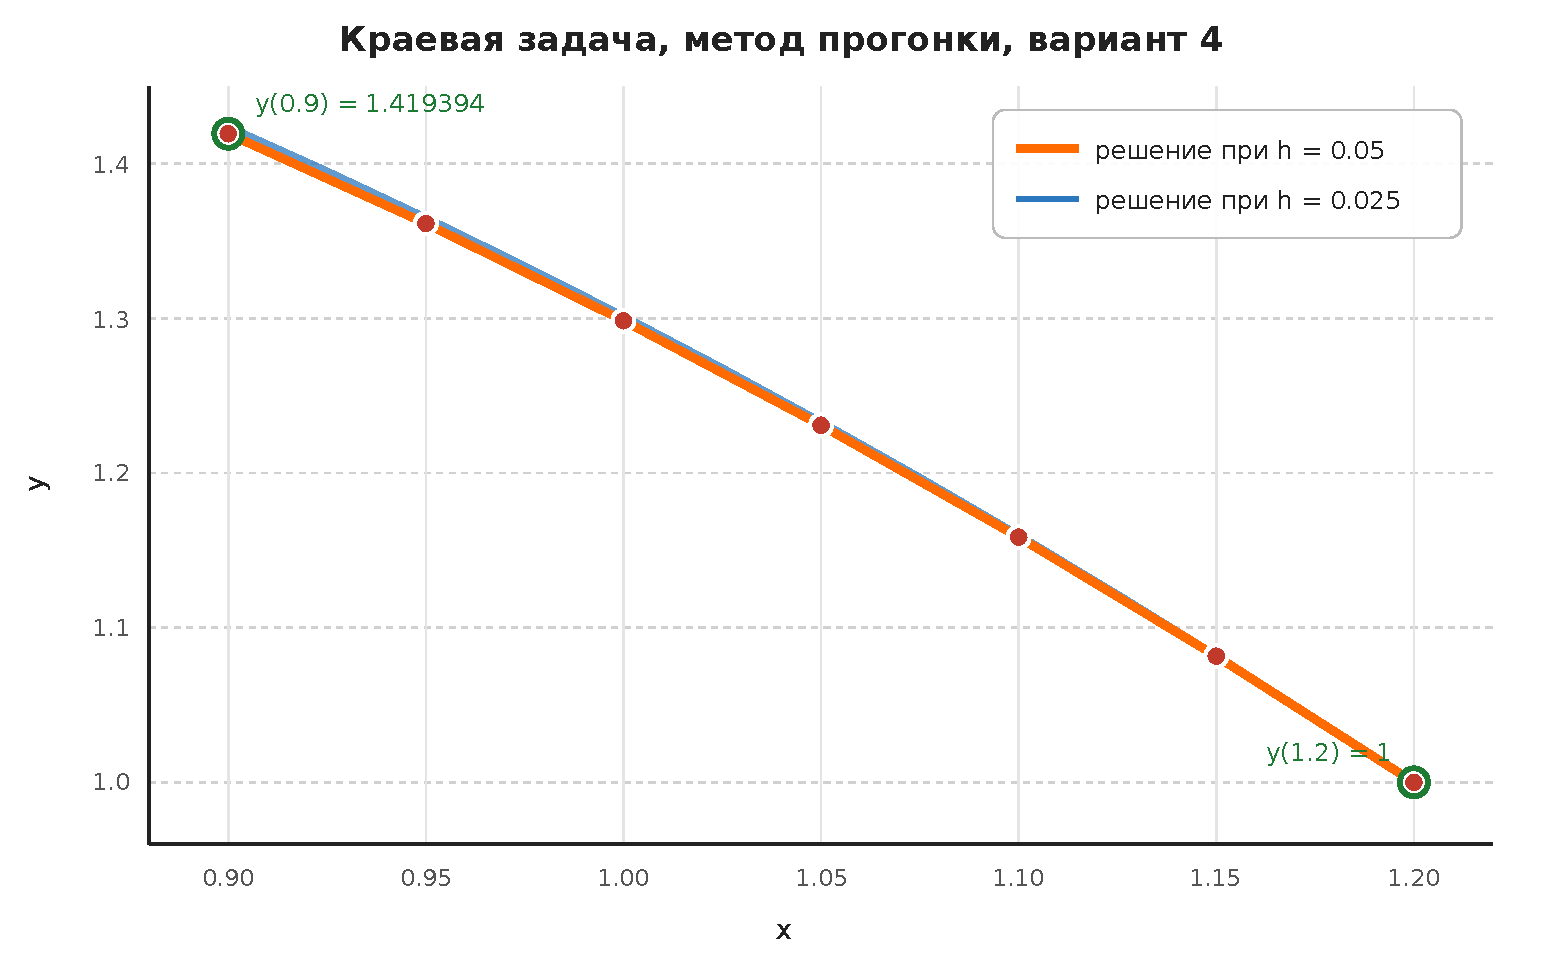
\includegraphics[width=0.9\textwidth]{fig_bvp.pdf}
    \caption{Решение краевой задачи методом прогонки, вариант~4}
    \label{fig:bvp}
\end{figure}

% =====================================================================
\section{Обсуждение результатов}
% =====================================================================

Метод прогонки дал монотонно убывающее решение: от $y(0{,}9)\approx1{,}4194$
до $y(1{,}2)=1$. Правое краевое условие ($\beta_1=0$) выполнено точно,
левое -- с погрешностью порядка $10^{-16}$. Максимальная невязка разностного
уравнения также не превышает $10^{-15}$ (см.~\eqref{eq:residual}), что
свидетельствует о правильности реализации алгоритма.

Внутренняя аппроксимация имеет порядок $O(h^2)$, однако краевые условия
заменены односторонними разностями порядка $O(h)$, поэтому суммарная
погрешность решения имеет первый порядок. Это подтверждается уточнением
решения при $x=0{,}9$: разности между последовательными сетками равны
$\approx5{,}13\cdot10^{-3}$ ($h\to h/2$), $\approx2{,}61\cdot10^{-3}$
($h/2\to h/4$) и $\approx1{,}32\cdot10^{-3}$ ($h/4\to h/8$), то есть
уменьшаются примерно вдвое при каждом измельчении сетки.

Программа использует ровно три одномерных массива: прогоночные
коэффициенты переиспользуются при переходе к более мелкой сетке,
а значения грубого решения сохраняются в части массива, не участвующей
в обратном ходе. Тем самым выполнено требование задания.

\end{document}
